%%%%%%%%%%%%%%%%%%%%%%%%%%%%%%%%%%%%%%%%%%%%%%
\section{Beamline}
\label{sec:h4beamline}

The H4 beamline will be extended to the NP04 cryostat in the newly constructed extension of EHN1. To produce particles in the momentum range of interest, the 80 GeV/c pion beam from the T2 primary target is sent onto a secondary target to generate a tertiary beam. Particles in the tertiary beam are momentum and charge-selected and transported down the H4 beamline extension into the protoDUNE detector. In principle the H4 beamline can operate in parallel with the H2 beamline. % minimize interference between the two ProtoDUNE experiments.

\subsection{H4 Beamline layout and optics}

A sketch of the H4 beamline extension layout is shown in Figure~\ref{fig:H4layout}. The first two dipole magnets (shown in red) after the secondary target are rotated by about 56$^\circ$ to move the beam downward towards the cryostat. The third dipole magnet (shown in green) is for sweeping the beam into one of the three beam windows.
\begin{cdrfigure}[H4 beamline layout]{H4layout}{Sketch of the H4 beamline layout in the region near the cryostat (Courtesy of V. Clerc, CERN).}
  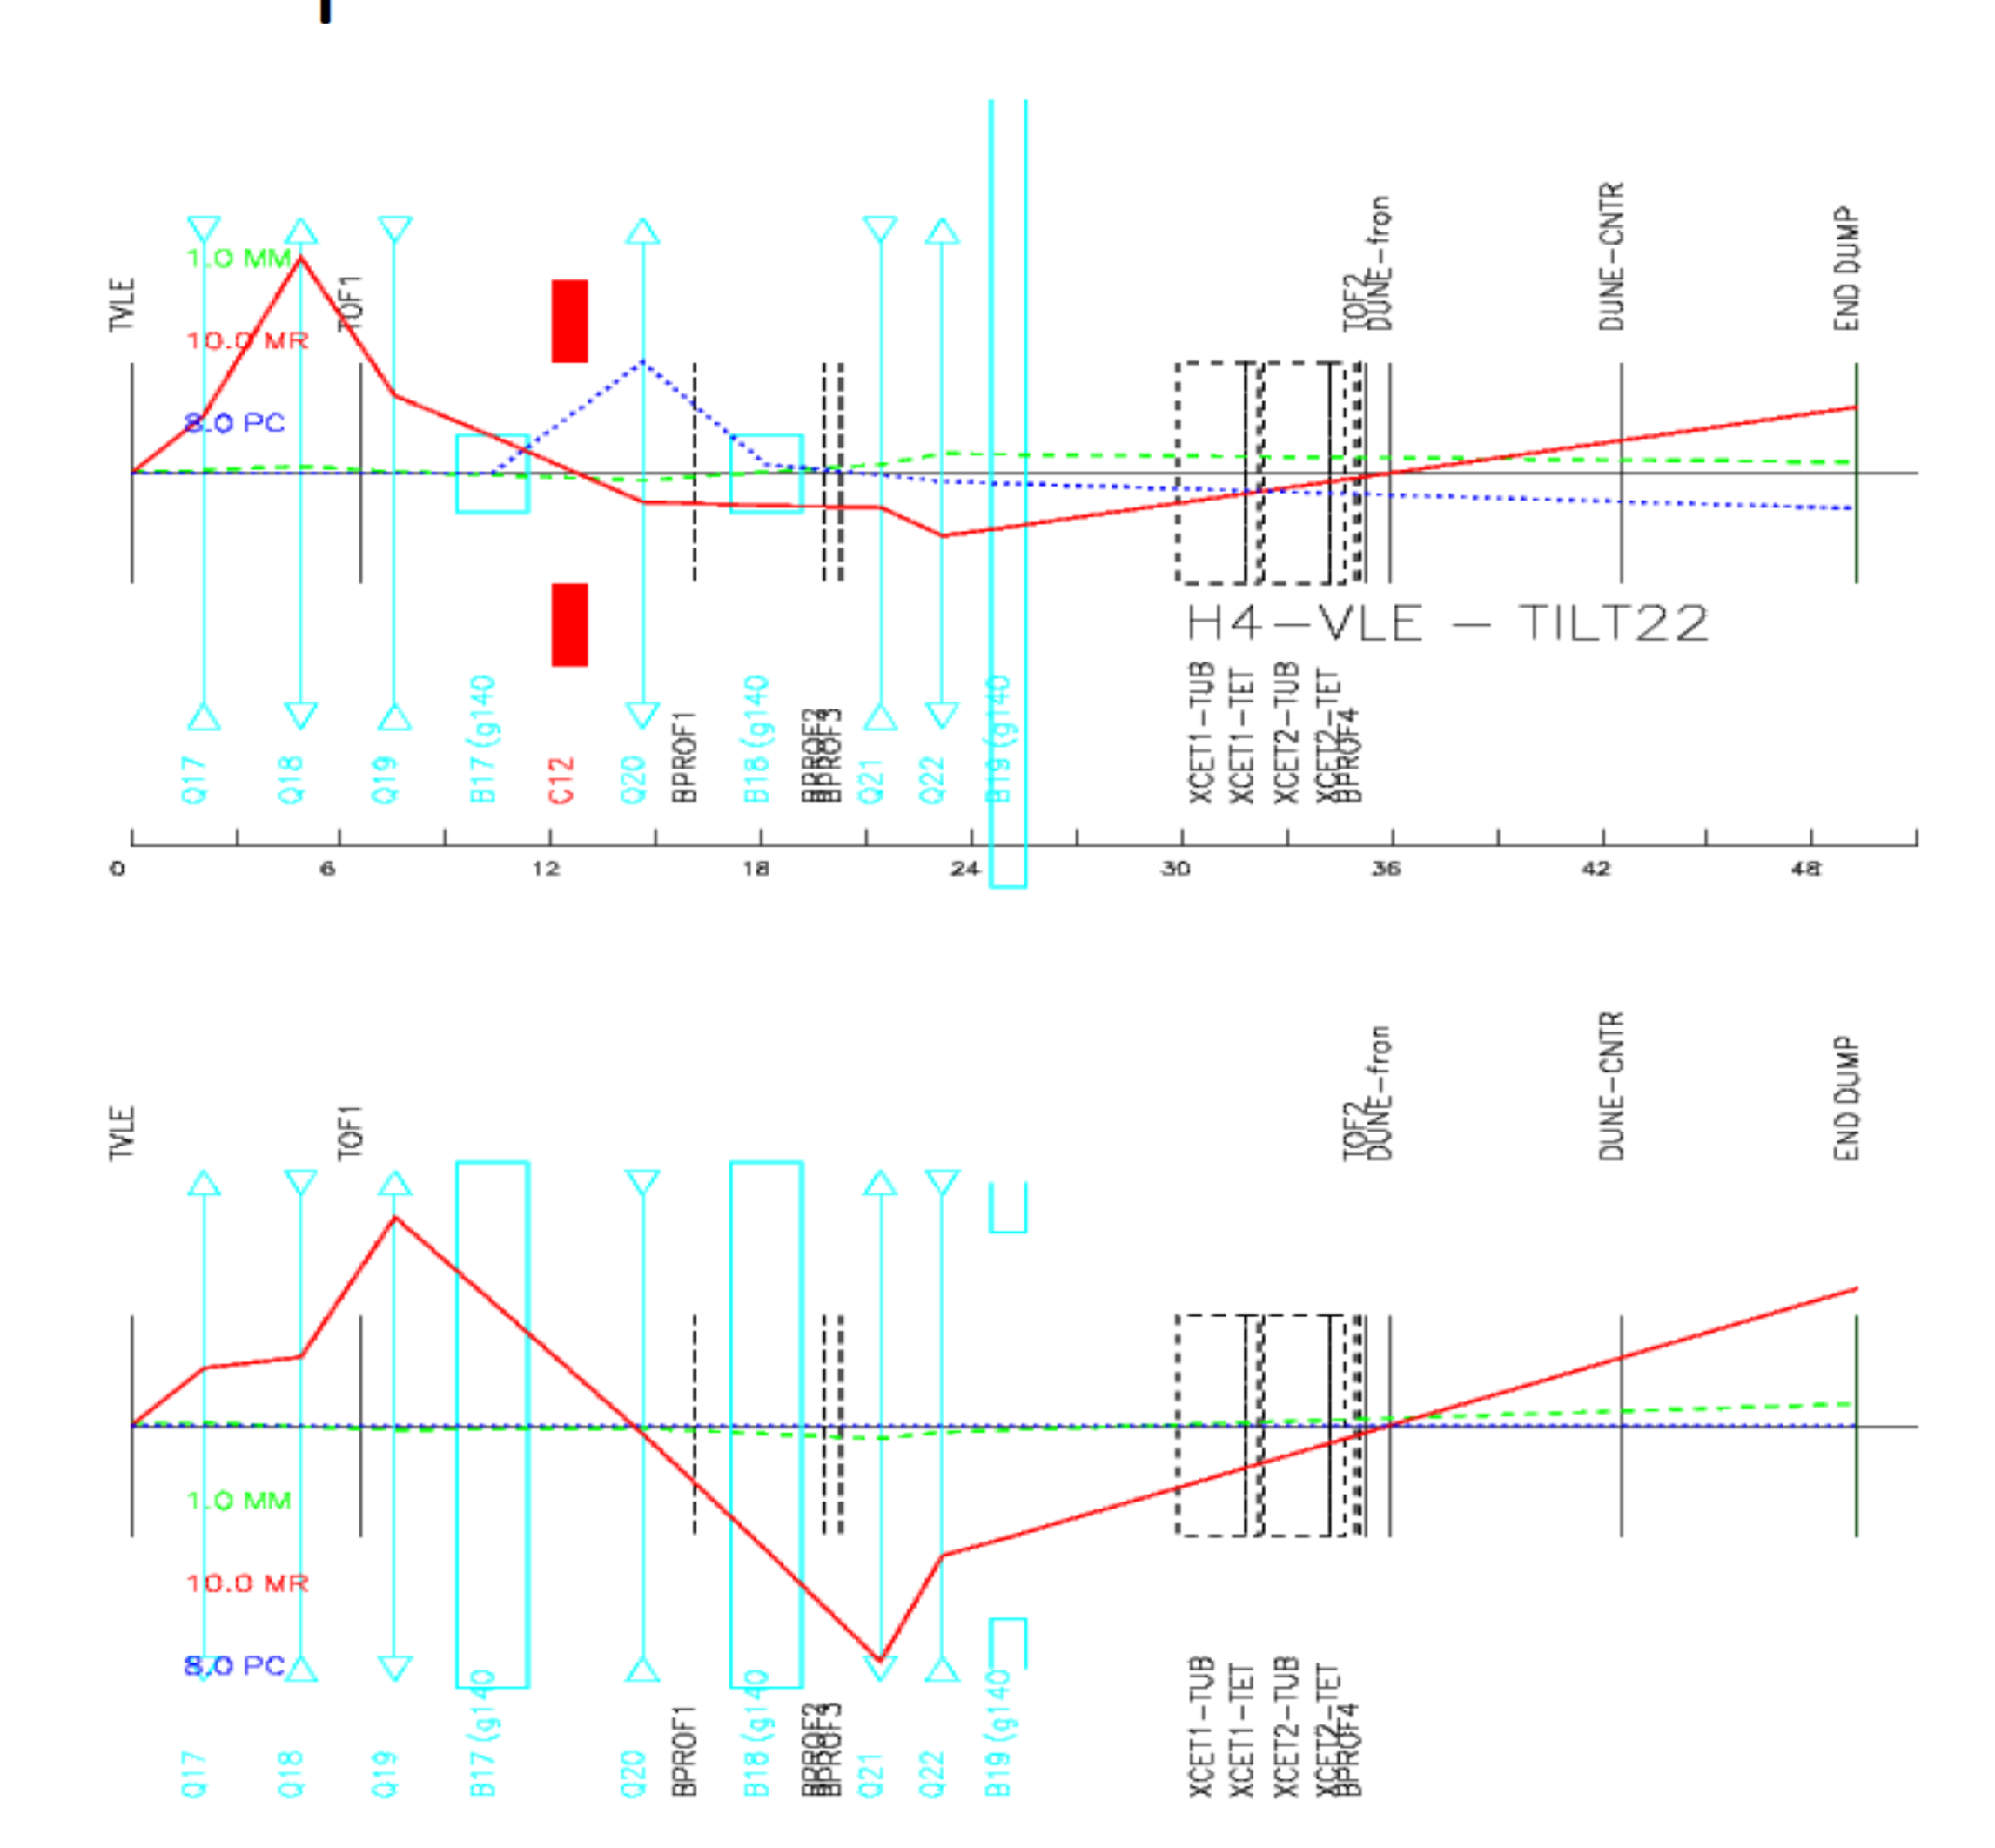
\includegraphics[width=0.75\textwidth]{beamline_H4layout.pdf}
\end{cdrfigure}


The beamline optics for the horizontal and vertical planes are shown in Figure~\ref{fig:beamoptics}. The series of dipole and quadropole magnets focus and direct the beam to one of the three beam windows. For the nominal configuration, the beam is focused at the front of the cryostat to ensure maximum acceptance of beam particle through the beam window penetration and the beam plug.

\begin{cdrfigure}[H4 beam optics]{beamoptics}{H4 beamline extension optics for the horizontal (top) and vertical (bottom) planes. The secondary target is located on the left side of the plots and the front of the ProtoDUNE-SP cryostat is located at the beam focus point, at about 33m from the secondary target. Q17-Q22 are the quadrapole magnets. B16 and B17 are the dipole bending magnets. BPROF1-4 are the beam profile monitors. XCET1 and XCET2 are the threshold Cherenkov counters. }
  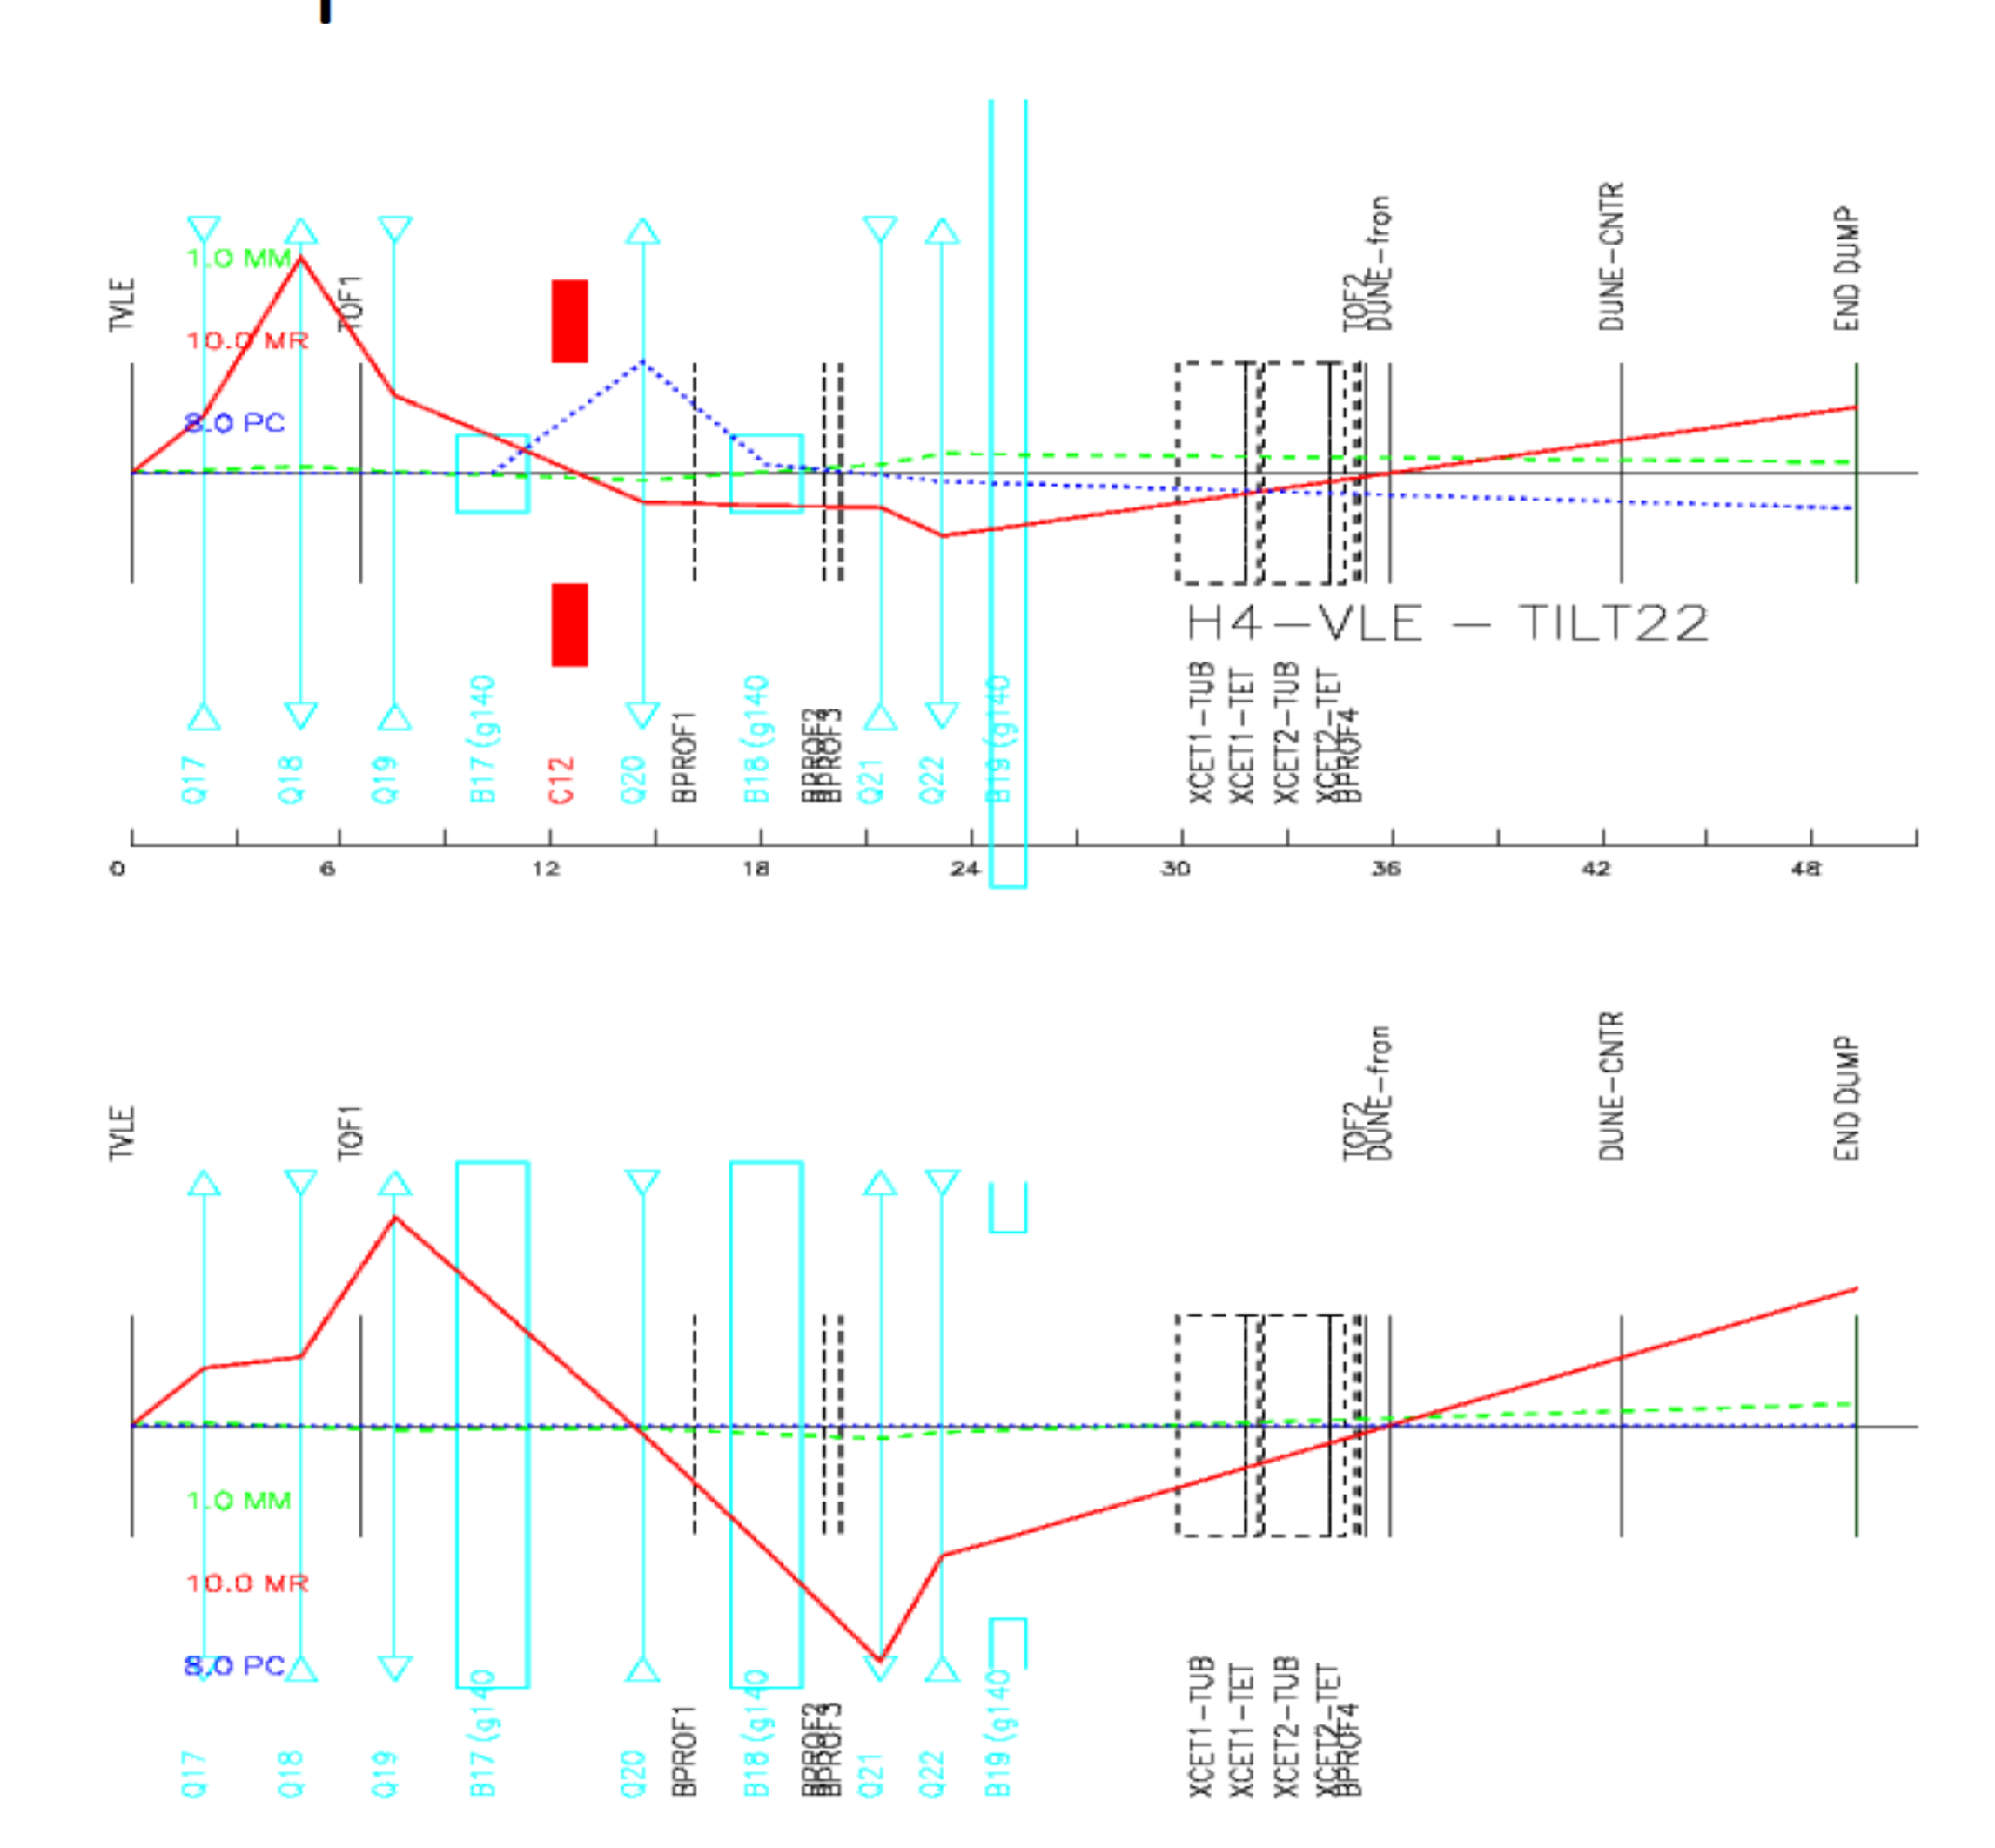
\includegraphics[width=0.99\textwidth, angle=-90]{beamline_H4Optics.pdf}
\end{cdrfigure}
\fixme{Need to update the beam optic diagram with the version that includes TOF}

\subsection{Beam properties}
%\fixme{Need simulation results from Nikos -- H4 beam files are available }
Recently, a full GEANT4 simulation of the H4 beamline including its extension to the protoDUNE cryostat has been performed \cite{H4beamfiles}. 
%%%Preliminary results based on the H4 beam line simulation are presented. 
The beamline model starts with the H4 secondary beamline 
%\fixme{does it also include the primary beam line ?}
to derive the particle properties in the tertiary beamline.  Target, magnets, collimators and a preliminary assumption
about beam instrumentation are included. The secondary target has been
modeled as a Tungsten cylinder (R=30mm, L=300mm) for beam particles with E$<3$GeV and as a Copper cylinder of the same dimensions  forbear particle energies  E$ge$3 GeV. Optimization of the target dimensions and material is ongoing.

Table \ref{tab:beampartcomp} describes the particle composition of the
beam at the entrance of the cryostat. Two features are evident. First, the beam is dominated by positrons at low energies,
and secondly, the kaon content, and to a lesser extent the pion content, are depleted at lower energies due to decays of these species 
along the beam path. 

%\fixme{add beam pipe radius in caption of table}
\begin{cdrtable}[Beam composition]{cccccc}{beampartcomp}{Beam composition (in percentage)  at the cryostat entrance for particles contained in the beam pipe (R= 10~cm).}
Momentum (GeV/c) & e$^+$ & $K^+$ & $\mu^+$ & p& $\pi^+$ \\ \toprowrule
1 & 69.7 & 0& 0.3 & 17.3 & 12.7\\ \colhline
2 &37.2& 0.6& 1.7& 24.1&36.3\\ \colhline
3 & 63.6&0.8&0.6&8.2&26.8\\ \colhline
4 & 46.4 & 1.8 & 1.1 & 8.5 & 42.1 \\ \colhline
5 &37.2 & 2.8 & 0.9 & 8.6 & 50.6\\ \colhline
6 &27.7 & 4.0 & 0.9& 10.2 & 57.3\\ \colhline
7 &20.7 & 4.8 & 1.0 & 10.7 & 62.8 \\
\end{cdrtable}
%%%%%%%%%%%%%%%%%%%%%%
Particle rates, assuming a spill intensity of $10^6$
particles on the secondary target and a SPS spill length of 4.8
seconds are reported in Table~\ref{tab:beampartrates}. 
%\fixme{What does "achievable" mean here ? e.g. is some special tweaking required to achieve these rates or is this some average coming out of the calculation.}
\begin{cdrtable}[Particle rate]{ccccccc}{beampartrates}{Particle rates (Hz).}
Momentum (GeV/c) & e$^+$ & $K^+$ & $\mu^+$ & p& $\pi^+$& total\\ \toprowrule
1 & 14 & 0 & 0 & 4 & 3  & 20 \\ \colhline
2 & 10 & 0 & 0 & 7 & 10 & 27 \\ \colhline
3 & 90 & 1 & 1 & 12 & 38 & 141\\ \colhline
4 & 68 & 3 & 2 & 12 & 61 & 146\\ \colhline
5 & 56 & 4 & 1 & 13 & 76 & 149\\ \colhline
6 & 47 & 7 & 1 & 17 & 97 & 169\\ \colhline
7 & 41 & 9 & 2 & 21 & 123& 196\\
\end{cdrtable}
%\fixme{Caption of table 7.3 says "trigger rates" whereas text says "particle rates". Unify language, I think it should be particle rates.}
%\fixme{what are the units for the rates in table 7.3 ?}

At momenta larger than about 4 GeV/c, the particle rates are in excess of  the
maximum acceptable rate, that is around
25-50~Hz. 
%\fixme{see earlier comment about max rate that the DAQ system may be able to cope with, e.g. 25 - 50Hz}
 At lower energies, the proton and pion rates are much lower, reduced by a
factor of 10 at 1 or 2 GeV/c, and are overwhelmed by the positron rate.

The momentum spread of the beam is of the order of 5 to 7 \%. At higher energies, where
the particle rate is higher, the momentum spread  can be narrowed by
closing the collimators, at the expense of the beam intensity.  For example, Figure \ref{fig:momcoll} shows
that at p=4~GeV/c the momentum uncertainty can be  reduced to $\Delta p/p= 3.6\%$ with a factor 4 reduction in particle rate.  
\begin{cdrfigure}[Beam momentum uncertainty]{momcoll}{Beam momentum uncertainty with different collimator openings at 4 GeV/c.}
  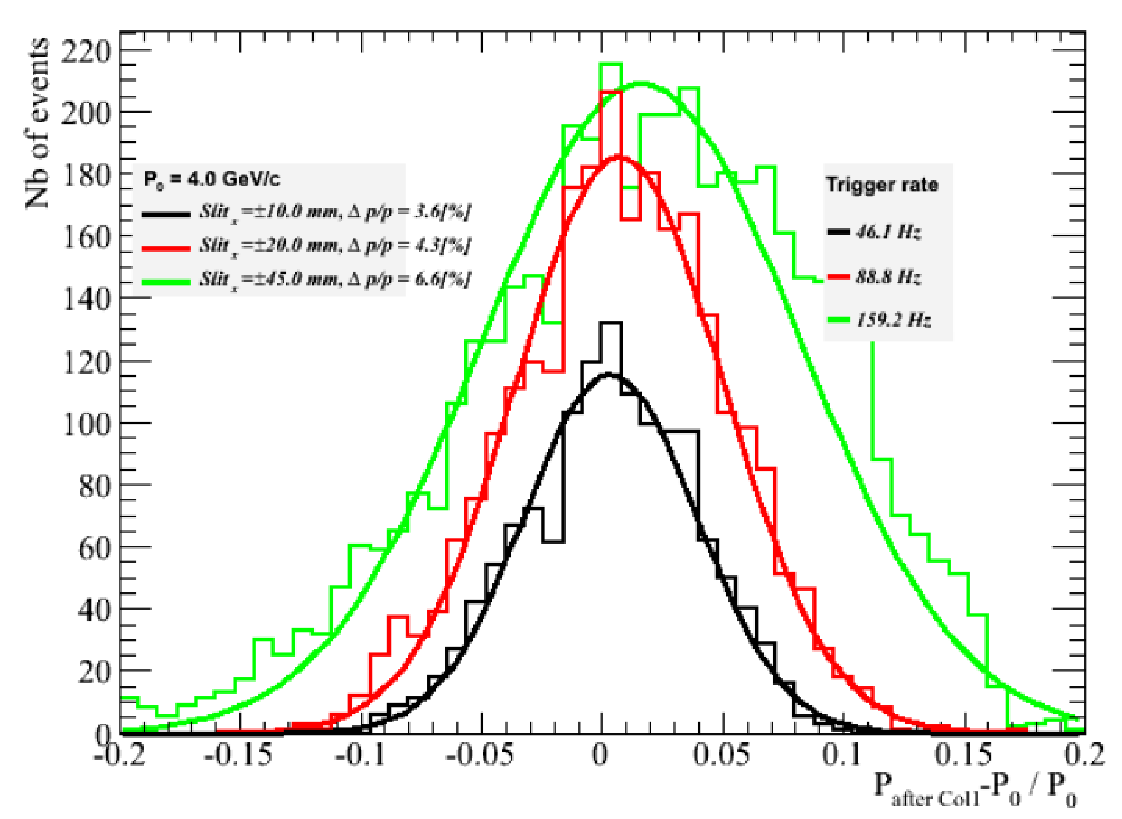
\includegraphics[width=0.75\textwidth]{Slits.pdf}
\end{cdrfigure}
\fixme{increase size of legend in figure; change trigger rate to particle rate in figure}
\fixme{How are the values of 3.6, 4.3 and 6.6\% obtained ? Not obvious from figure.}
\fixme{ Figure from Nikos, need him to redo it}


\subsection{Muon halo}
The secondary beam is mainly composed of 80 GeV pions. In the long path ($\approx$ 600~m) between the primary and the secondary target,
%\fixme{add (approximate) distance in m }
 an intense high energy muon halo is produced by pion decay. Muons propagate approximately in the direction of the first section of the H4 beamline, 
%%% \fixme{It may be useful to distinguish explicitly between H4 beam line and H4 beam line extension. Earlier the beam line pointing downwards towards the cryostat was also referred to as H4 beam line.}
 that is slightly upward of the H4 beam line extension which points at the protoDUNE SP detector.  
 Therefore the most intense part of the muon halo passes 1 to 2 metres above the ProtoDUNE SP cryostat. 
% \fixme{Can we add an approximate distance in m ?}
Figure \ref{fig:muonhalo_HE} shows the spatial distribution of the muon halo at the face of the cryostat. Only muons with momentum larger than 4~GeV/c have been considered. Despite the low statistics of the simulations, the up-down asymmetry is clearly visible. The origin of the coordinate system is chosen to coincide with the center of the cryostat face. The color scale shows the muon intensity in $\mu /m^2/spill$ for $10^6$ particles/spill from the primary target. The muon intensity on the cryostat face ranges from 1 to 400  $\mu /m^2/spill$.
Fig. \ref{fig:muonhalo_HE}  is very preliminary, not only because of low statistics, but also because shielding around the low energy beam line is not included in the simulation, and the muons produced in neighboring beamlines in H1N1, including the H2 line that feeds the DualPhase ProtoDUNE, are not considered here. 
\begin{cdrfigure}[Muon halo intensity at the cryostat face]{muonhalo_HE}{Muon halo intensity at the cryostat face for muons originating from the H4 beam line and with $P_\mu  \ge 4$~Gev/c. The origin of the coordinate system is centered on the cryostat and dimensions are in mm. Color scale is in units of $\mu /m^2/spill$. The black and red rectangles represent the cryostat face and the active detector volume}
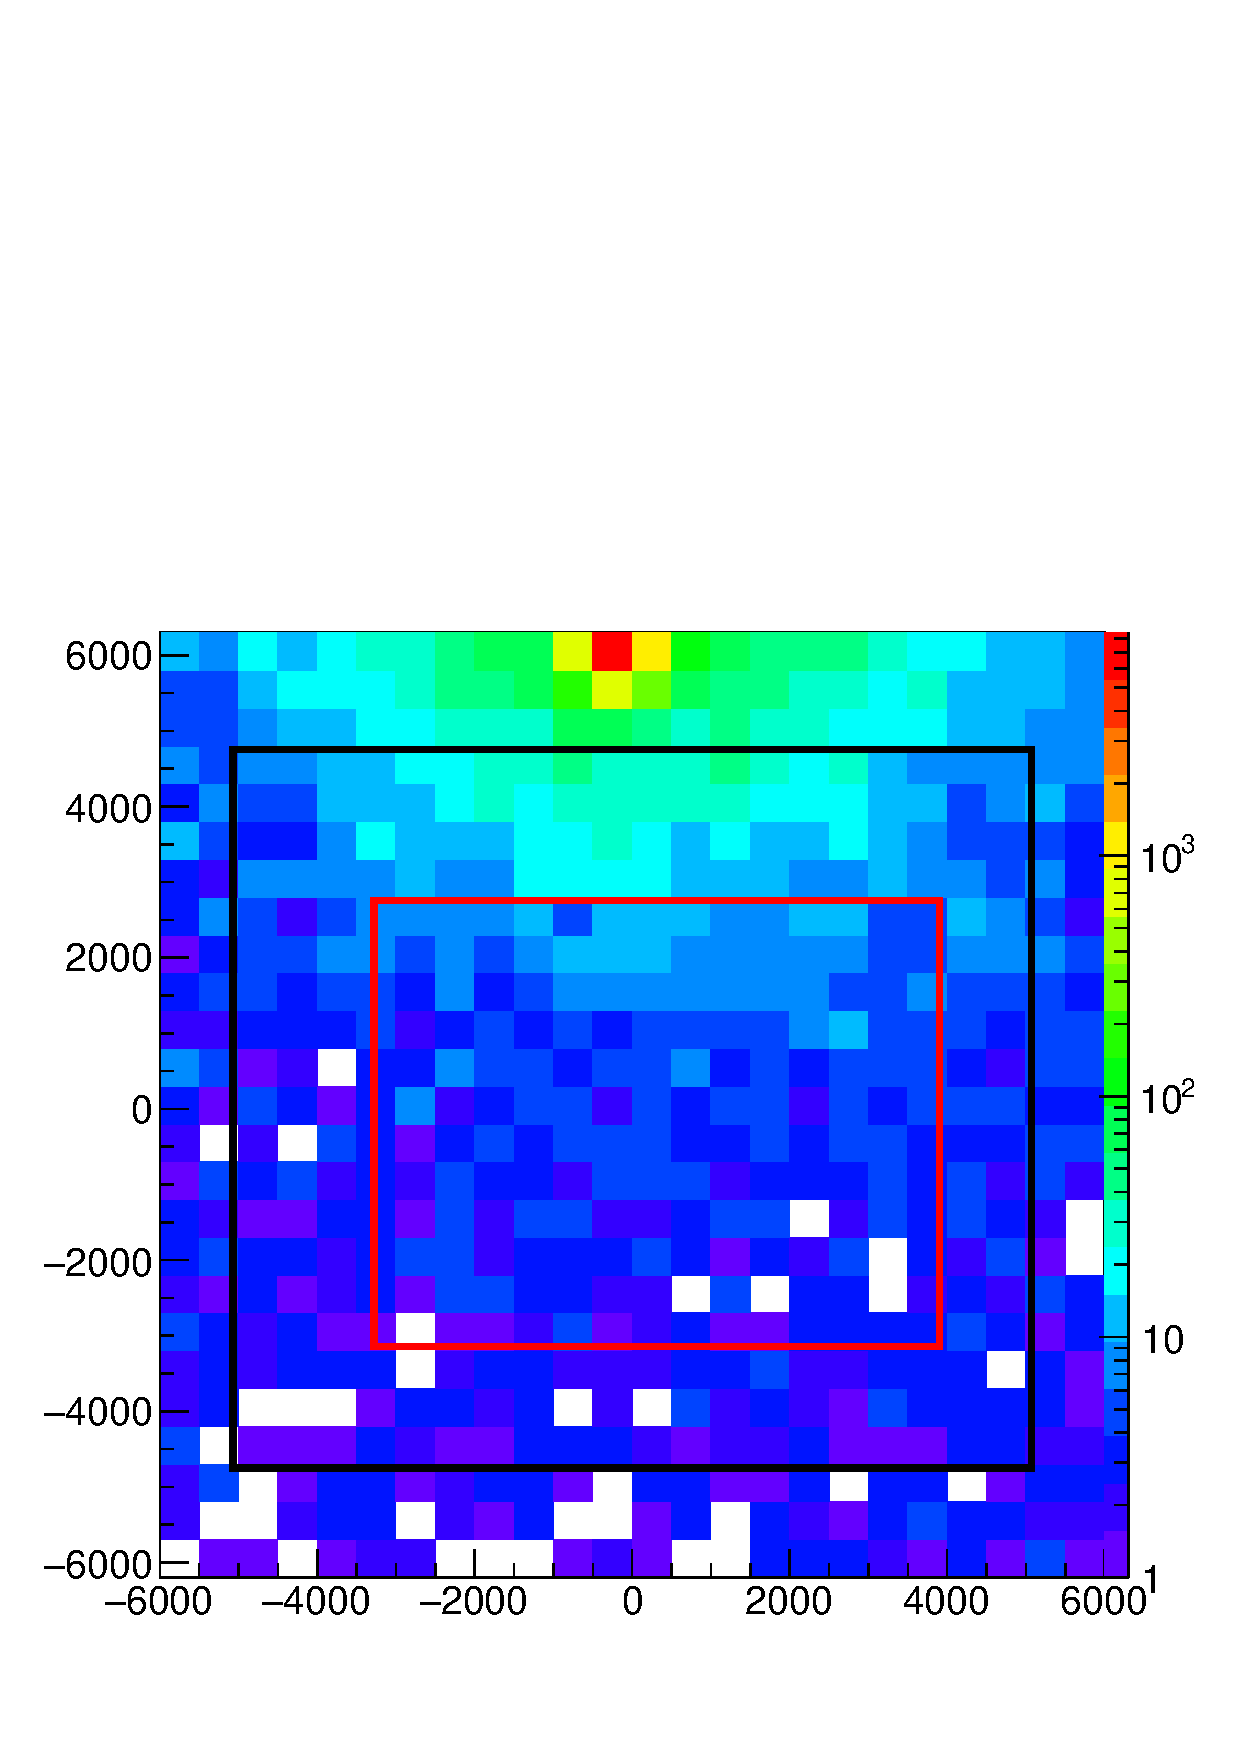
\includegraphics[width=0.50\textwidth]{muon_map_HE_square.pdf}
\end{cdrfigure}
%\fixme{Fig. 7.5: add axes labels; superimpose two rectangles one showing cryostat face and second showing active detector volume.Exponents on color scale are cut off}




